\begin{enumerate}
\item Le signe « point » vaut $1$ (on peut le déduire des $3$ points valant $3$) et le signe « trait » vaut $4$.
\item Le nombre 21 s’écrit :

\medskip
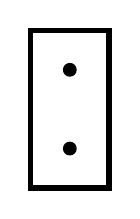
\begin{tikzpicture}[x=1cm,y=1cm]
\draw[line width=2pt] (-6,3) -- (-5,3) -- (-5,1) -- (-6,1) -- cycle;
\begin{scriptsize}
\fill (-5.5,1.5) circle (2.5pt);
\fill (-5.5,2.5) circle (2.5pt);
\end{scriptsize}
\end{tikzpicture}

\item $37 = 1 \times 20 + ( 2 + 3 \times 5)$ donc un signe « point » sur la première ligne puis $2$ signes «  point »  et $3$ signes « trait »
\item 
\begin{minipage}{7cm}
\begin{enumerate}
	\item \includegraphics[width=.1\textwidth]{./images/2022-g2-ex5-img3.png}
	
	Ce nombre est égal à :
	
	$3 \times 20 + (4 + 2 \times 5 ) = 60 + 4 + 10 = 74$
\end{enumerate}
\end{minipage}
\begin{minipage}{9cm}
\begin{enumerate}
	\setcounter{enumii}{1}
	\item \includegraphics[width=.1\textwidth]{./images/2022-g2-ex5-img4.png}
	
	Ce nombre est égal à :
	
	$1 \times 20^2 + (2 + 3 \times 5) \times 20 + 5 = 400 + 17 \times 20 + 5 = 745$
\end{enumerate}
\end{minipage}
\item 
\begin{enumerate}
	\item $25=1\times 20 + 5$.
	
\medskip
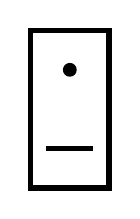
\begin{tikzpicture}[x=1cm,y=1cm]
\draw[line width=2pt] (-6,3) -- (-5,3) -- (-5,1) -- (-6,1) -- cycle;
\begin{scriptsize}
\fill (-5.5,2.5) circle (2.5pt);
\draw[line width=2pt] (-5.8,1.5) -- (-5.2,1.5);
\end{scriptsize}
\end{tikzpicture}

	\item $101 = 2\times 5\times 20 +1 $.

\medskip
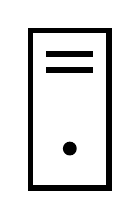
\begin{tikzpicture}[x=1cm,y=1cm]
\draw[line width=2pt] (-6,3) -- (-5,3) -- (-5,1) -- (-6,1) -- cycle;
\begin{scriptsize}
\fill (-5.5,1.5) circle (2.5pt);
\draw[line width=2pt] (-5.8,2.5) -- (-5.2,2.5);
\draw[line width=2pt] (-5.8,2.7) -- (-5.2,2.7);
\end{scriptsize}
\end{tikzpicture}
	
	\item La position d’un signe dans l’écriture du nombre change sa valeur. Ainsi un signe « point » peut valoir $1$ ou valoir $20$. 
\end{enumerate}
\end{enumerate}